\begin{savequote}[75mm]
More and more I find that in order to create effectively one has to consider delirium and, yes, organize it.
\qauthor{Pierre Boulez\footnote{\citet[144]{boulez-quote}}}
\end{savequote}

\chapter{\textit{Polillas} (2021) for String Quartet}
\label{Chapter3}
% \lettrine[lines=2,slope=-2pt,nindent=2pt]{\textcolor{SchoolColor}{P}}{olillas, my third string quartet,}

\lettrine[lines=3]{\setmainfont{GoudyInitialen}[Path=./fonts/, Extension = .ttf]\color{printGreen}P}{olillas, my third string quartet,} was deeply influenced by the preceding works. While my previous compositions featured distinct materials, this was the first work in which I incorporated formalized manifestations of each material and variegated formal structures. In fact, this work plays out as a dialogue between \textit{sequential sectionality} and \textit{variegated sectionality} because the first half of the work features a great deal of material polyphony, while the second half comprises mostly \textit{oppositional} material juxtapositions. This quartet alludes to both \textit{Rhea} and \textit{Akasha} in several explicit ways, both subtle and straightforward.


\section{Inherited Techniques}

Some aspects of my compositional process are inherited directly from the aforementioned composers. Since 2018 all of my instrumental compositions have been implemented through the use of Trevor Bača's Abjad \ac{API}. As a result, I have had access to many of the techniques employed in his works. For instance, all of the rhythmic material in my pieces have used the \textit{rmakers} library described in \vref{rmakers}. Also much of the data processing in my work is performed with the Abjad \textit{Sequence} library as well as \emph{many} of my own functions and classes.

\subsection{Storyboarding}

In preparation for this piece, I defined various materials and their available manifestations. The permutations and distribution of materials in the piece were performed abstractly, before the materials had crystallized into their final forms, but the large-scale form and the basic materials cyclically informed one another. Finally, I produced a nearly complete storyboard in both a text and color-map. This measure-by-measure catalog of events did not originally include the lengths of any of the measures. In my process, I like to keep some aspect of the work a ``surprise'' until I am realizing my sketches as a final, notated document. Every time signature is derived from a formalized procedure, however no decision was based on their lengths until the last possible moment.

\subsection{Time Signature Helianthation}

A technique I chose to use in \textit{Polillas} which came directly from \textit{Akasha} was the use of alternating time signature series derived from helianthations of nested numerator sequences. Just like \textit{Akasha}, the generative process for each series is defined then each series is subsequently rotated for every compositional segment at regular rotation intervals. However, in the case of \textit{Akasha}, rotations were performed on the nested helianthations, but in \textit{Polillas} rotations are performed by individual numerators. I also adopted Bača's tendency in the helianthation technique to configure the helianthations with reversed rotations of $(-1, 1)$ and monotonically increase or decrease the integers in each sub-list. Each series is either increasing or decreasing. This, in combination with the ability for the rhythm makers\footnote{See \vref{rmakers}.} to produce output based on input durations, causes segments which use series A or C to have phrases which generally rallantando and segments which use series B to have accelerating elements. The time signature series to be used within a given segment is ordered by the following cyclic permutations [[A, B, C], [A, C, B], [B, A, C], [B, C, A], [C, A, B], [C, B, A]]. Thus, segment 1 uses series A, segment 2 uses B, segment 3 uses C, segment 4 uses A, segment 5 uses C, and so on, looping back to the beginning of the cycle when the number of segments exceeds the number of permuted values.

\begin{lstlisting}[language=Python,frame=tb,caption={Generating processes for time signatures in Polillas},label=lst:p-sigs]
time_signature_series = dict()

numerators = evans.Sequence([[3, 4, 4], [3, 5, 6], [7]])
groups = numerators.helianthate(-1, 1)
numerators = evans.Sequence(groups).flatten(depth=-1)
_time_signatures = [abjad.TimeSignature((_, 4)) for _ in numerators]
groups = evans.Sequence(_time_signatures)
time_signature_series["A"] = groups  # -2 cycles

numerators = evans.Sequence([[9, 8, 7, 7], [8, 6, 6], [5, 4, 3]])
groups = numerators.helianthate(-1, 1)
numerators = evans.Sequence(groups).flatten(depth=-1)
_time_signatures = [abjad.TimeSignature((_, 8)) for _ in numerators]
groups = evans.Sequence(_time_signatures)
time_signature_series["B"] = groups  # -3 cycles

numerators = evans.Sequence([[5, 6, 8], [10, 11, 12], [12, 13, 13, 15], [14, 16]])
groups = numerators.helianthate(-1, 1)
numerators = evans.Sequence(groups).flatten(depth=-1)
_time_signatures = [abjad.TimeSignature((_, 16)) for _ in numerators]
groups = evans.Sequence(_time_signatures)
time_signature_series["C"] = groups  # -1 cycles
\end{lstlisting}

\subsection{Series A}

Time signature series A is defined as the sequence $[[3, 4, 4], [3, 5, 6], [7]]$ always over a denominator of \lilyText{4} but occasionally signatures are replaced with \lilyTimeSignature{1}{6} to disrupt the polyrhythmic material (described in \vref{material-C-summary}). This series rotates in cycles of +2 of the flattened helianthations for each of the segments in which it appears.

\begin{lstlisting}[language=Python,frame=tb,caption={Enumeration of helianthated rotations of time signature series A in Polillas},label=lst:p-sigs-a]
>>> import evans
>>> numerators = evans.Sequence([[3, 4, 4], [3, 5, 6], [7]])
>>> groups = numerators.helianthate(-1, 1)
>>> for group in groups:
...     print(group)
...
[3, 4, 4]
[3, 5, 6]
[7]
[7]
[4, 4, 3]
[5, 6, 3]
[6, 3, 5]
[7]
[4, 3, 4]
\end{lstlisting}

\subsection{Series B}

Time signature series B is defined as the sequence $[[9, 8, 7, 7], [8, 6, 6], [5, 4, 3]]$ always over \lilyText{8}. Rotations are performed in cycles of +3 of the flattened helianthations.

\begin{lstlisting}[language=Python,frame=tb,caption={Enumeration of helianthated rotations of time signature series B in Polillas},label=lst:p-sigs-b]
>>> numerators = evans.Sequence([[9, 8, 7, 7], [8, 6, 6], [5, 4, 3]])
>>> groups = numerators.helianthate(-1, 1)
>>> for group in groups:
...     print(group)
...
[9, 8, 7, 7]
[8, 6, 6]
[5, 4, 3]
[4, 3, 5]
[8, 7, 7, 9]
[6, 6, 8]
[6, 8, 6]
[3, 5, 4]
[7, 7, 9, 8]
[7, 9, 8, 7]
[8, 6, 6]
[5, 4, 3]
\end{lstlisting}

\subsection{Series C}

Time signature series C is defined as the sequence $[[5, 6, 8], [10, 11, 12], [12, 13, 13, 15], [14, 16]]$ always over \lilyText{16} with rotations in cycles of +1. \vspace{0.5cm}

\begin{lstlisting}[language=Python,frame=tb,caption={Enumeration of helianthated rotations of time signature series C in Polillas},label=lst:p-sigs-c]
>>> numerators = evans.Sequence([[5, 6, 8], [10, 11, 12], [12, 13, 13, 15], [14, 16]])
>>> groups = numerators.helianthate(-1, 1)
>>> for group in groups:
...     print(group)
...
[5, 6, 8]
[10, 11, 12]
[12, 13, 13, 15]
[14, 16]
[16, 14]
[6, 8, 5]
[11, 12, 10]
[13, 13, 15, 12]
[13, 15, 12, 13]
[14, 16]
[8, 5, 6]
[12, 10, 11]
[10, 11, 12]
[15, 12, 13, 13]
[14, 16]
[5, 6, 8]
\end{lstlisting}

After defining the process by which time signatures are arranged in each segment, the number of measures for each segment is chosen. If the number of measures in a segment is greater than the number of available the time signatures loop from the beginning until all measures are assigned a meter, exactly as is done in \textit{Akasha}. Some measures are selected by index to be a silent grand pause. The original time signature of each fermata measure is completely removed, which is different than \textit{Akasha}'s fermata insertion process. From this blank score page, I begin to transfer my measure-by-measure, text-based storyboard and graphic material timeline of the piece into notation.

\subsection{Rhythm makers}

In previous pieces, my use of the rhythm makers was somewhat generic, but similar to Guerrero's rhythmic techniques. A rhythm maker would be configured and applied to every instance of a given material within a specific segment. With a state-management system, the process of a rhythm maker would begin in another voice where it had left off in a previous voice. This produced unified textures across an ensemble, but allowed for little directional development. In Polillas, I adopted the approach seen in \textit{Akasha}. Rhythmic behaviors are more unique and configured by hand in each moment. Three insteresting examples can be seen in the 4\textsuperscript{th} segment which begins at measure 61. The materials presented in this segment are materials \boxed{\text{A}}, \boxed{\text{F}}, and \boxed{\text{E}}.

In this case, the rhythms of \boxed{\text{A}} make use of the rhythm tree\footnote{IRCAM's implementation of rhythm trees in the OpenMusic software is known as RTM.} parser found in Abjad. Two different rhythm trees are subjected to a two part helianthation process. These two sequences are then combined into one long cyclic sequence. Each rhythm tree is applied to a single measure.

\begin{lstlisting}[language=Python,frame=tb,caption={Stage 1 of material A rhythms in Polillas},label=lst:p-a-rhythm]
def shadows(
    extra_counts=[2], stage=3, preprocessor=None, rewrite=False, rewrite_boundary=None
): 
    if stage == 1:
        rtm_strings_1 = evans.helianthated_rtm(
            beats=[[3], [1, 1], [2, 1]],
            divisions=[[1], [1, 1, 1], [2, 1, 1]],
        )
        rtm_strings_2 = evans.helianthated_rtm(
            beats=[[2], [1, 2], [3, 1]],
            divisions=[[1, 1], [1, 1, 1], [1, 2]],
        )
        rtm_strings = rtm_strings_1 + rtm_strings_2
        maker = evans.RTMMaker(rtm_strings)
        commands = [
            maker,
            rmakers.trivialize(lambda _: abjad.select.tuplets(_)),
            rmakers.rewrite_rest_filled(lambda _: abjad.select.tuplets(_)),
            rmakers.extract_trivial(),
        ]
        if rewrite is True:
            commands.append(evans.RewriteMeterCommand(boundary_depth=rewrite_boundary))
        stack = rmakers.stack(*commands, preprocessor=preprocessor)
        handler = evans.RhythmHandler(stack, forget=False)
        return handler
\end{lstlisting}

The helianthation function rotates the rhythm trees in a process reminiscent of Brian Ferneyhough's rhythm tree rotations found in his \textit{String Trio}. A rhythm tree can be considered by each layer independently. In the case of this function, I constrain the process to trees of only two layers, but it could be extrapolated to arbitrary nesting. The first layer of the tree partitions the measure into divisions and the second layer partitions the divisions into subdivisions. Unlike Ferneyhough's rotations, which rotate the integers of all layers simultaneously, two helianthations direct each layer of the rotation process independently.

\begin{lstlisting}[language=Python,frame=tb,caption={RTM Helianthation Function},label=lst:rtm-helianthation]
def helianthated_rtm(
    divisions, beats, divisions_rotations=(-1, 1), beats_rotations=(-1, 1)
):
    s = Sequence(divisions).helianthate(divisions_rotations[0], divisions_rotations[1])
    s_ = Sequence(
        flatten(Sequence(beats).helianthate(beats_rotations[0], beats_rotations[1]))
    )
    c_s_ = CyclicList(s_, forget=False)
    beats = c_s_(r=len(s))
    out_ = []
    for x, y in zip(beats, s):
        temp = [x, y]
        out_.append(temp)
    out = Sequence(out_).partition_by_counts(
        [len(divisions)], cyclic=True, overhang=True
    )
    final_out = []
    for rtm_list in out:
        final_temp = [1, rtm_list]
        final_out.append(final_temp)
    rtm_out = []
    for _ in final_out:
        rtm = nested_list_to_rtm(_)
        rtm_out.append(rtm)
    return rtm_out
\end{lstlisting}

The user inputs values as nested lists. Each layer is rotated in opposite directions resulting in two unique sequences. The divisions are grouped into a flattened sequence of the length of the original sequence.\footnote{For instance if the original sequence was [[3], [1, 1], [2, 1]], then the list of divisions would be [3, 1, 1, 2, 1 ...] which is subsequently re-partitioned to groups of three (i.e. [3, 1, 1], [2, 1, 1] etc.).} Then each group of subdivisions is nested within each division. Theoretically each helianthated sequence has a different length, therefore the subdivisions are cyclically applied to the length of the list of divisions. This process produces a mass texture with intermittent tension and release in the form of dense packets of rhythmic values alternating with longer durations.

The rhythms for material \boxed{\text{F}} are similar to rhythms found in \textit{Akasha}. The input measures are pre-processed, fused and/or split into divisions of different size. In this segment, some pre-processing produces groups of 2 quarters followed by 1 quarter note, while other passages pre-process to only groups of 2 quarters. Sequences of extra counts are input to a talea of 16\textsuperscript{th} notes to increase or decrease the number of attacks per moment. All leaves are forced to rests, but select leaves are turned back into leaves by a user-input sequence of indices and a period of repetition. After the sounding leaves are reintroduced, another user-input sequence of indices with a period of repetition is used to silence entire tuplets.

\begin{lstlisting}[language=Python,frame=tb,caption={Stage 4 of material F rhythms in Polillas},label=lst:p-f-rhythm]
def knots(
    stage=1,
    extra_counts=None,
    division_indices=[0],
    leaf_indices=[0, 2, 3],
    leaf_period=7,
    rotation=0,
    preprocessor=None,
    rewrite=False,
    rewrite_boundary=None,
):
    if stage == 4:
        def selector(_):
            sel_1 = abjad.select.leaves(_)
            sel_2 = abjad.select.get(sel_1, leaf_indices, leaf_period)
            return sel_2
        attack_selector = selector
        def division_selector(selections):
            sel_1 = abjad.select.tuplets(selections)
            sel_2 = abjad.select.get(sel_1, division_indices)
            return sel_2
        commands = [
            rmakers.talea(
                [1],
                16,
                extra_counts=extra_counts,
            ),
            rmakers.force_rest(lambda _: _),
            rmakers.force_note(attack_selector),
            rmakers.force_rest(division_selector),
            rmakers.trivialize(lambda _: abjad.select.tuplets(_)),
            rmakers.rewrite_rest_filled(lambda _: abjad.select.tuplets(_)),
            rmakers.rewrite_sustained(lambda _: abjad.select.tuplets(_)),
            rmakers.extract_trivial(),
        ]
        if rewrite is True:
            commands.append(evans.RewriteMeterCommand(boundary_depth=rewrite_boundary))
        stack = rmakers.stack(*commands, preprocessor=preprocessor)
        handler = evans.RhythmHandler(stack, forget=True)
        return handler
\end{lstlisting}

The rhythms for material \boxed{\text{E}} uses a tuplet rhythm maker to partition divisions of each measure into tuplets of the proportions $(3, 1)$. These tuplets are used as anchor points for crescendo hairpins. The cello features a special alternative to this process where every other rhythm application is given a single attack instead of a tuplet.\footnote{This special cello version is used in the previous segment, number 3, not the segment currently being discussed.}

\begin{lstlisting}[language=Python,frame=tb,caption={Stage 1 of material E rhythms in Polillas},label=lst:p-e-rhythm]
def chilled(
    stage=3,
    extra_counts=None,
    input_counts=None,
    reverse=False,
    rotation=0,
    preprocessor=None,
    rewrite=False,
    rewrite_boundary=None,
):
    if stage == 1:
        commands = [
            rmakers.tuplet([(3, 1)]),
            rmakers.trivialize(lambda _: abjad.select.tuplets(_)),
            rmakers.rewrite_rest_filled(lambda _: abjad.select.tuplets(_)),
            rmakers.rewrite_sustained(lambda _: abjad.select.tuplets(_)),
            rmakers.extract_trivial(),
        ]
        if rewrite is True:
            commands.append(evans.RewriteMeterCommand(boundary_depth=rewrite_boundary))
        stack = rmakers.stack(*commands, preprocessor=preprocessor)
        handler = evans.RhythmHandler(stack, forget=True)
        return handler
    if stage == "1 cello":
        commands = [
            rmakers.tuplet([(3, 1), (1,)]),
            rmakers.trivialize(lambda _: abjad.select.tuplets(_)),
            rmakers.rewrite_rest_filled(lambda _: abjad.select.tuplets(_)),
            rmakers.rewrite_sustained(lambda _: abjad.select.tuplets(_)),
            rmakers.extract_trivial(),
        ]
        if rewrite is True:
            commands.append(evans.RewriteMeterCommand(boundary_depth=rewrite_boundary))
        stack = rmakers.stack(*commands, preprocessor=preprocessor)
        handler = evans.RhythmHandler(stack, forget=True)
        return handler
\end{lstlisting}

\subsection{Pitch}

The use of pitch in \textit{Polillas} takes a more formalized approach than \textit{Akasha}. While the harmonic material in \textit{Akasha} is clearly coupled with the rhythmic processes of each material, most of the pitches are input into the section files by hand. In Polillas, more concrete systems are established for the proliferation of pitch materials. In situations when there is no generating function deployed in a segment, this means a chord sequence had been generated as a part of the sketch process. For these progressions, voice-leading was performed by hand then input directly into each relevant segment file.

In previous pieces, I modeled idiomatic voice-leading through the use of Brownian Motion. This was partly a result of my studies of the music of Alberto Posadas and Francisco Guerrero whose music features Brownian motion on several parameters, but most frequently in pitch space. I would typically produce a large, vertical chord with some specific property, such as Elliott Carter's ``Link'' chords, all-interval twelve-tone rows with one contiguous instance of the all-trichord hexachord, voiced as a harmony rather than a tone row. For each voice in the ensemble, I would constrain the chord to the register of each instrument and I would map a random walk onto the chord to produce the melodic sequence of a segment of music. In my first string quartet, \textit{Hamonshū}, there were four basic chords which underwent a process of compression and expansion. The piece began with the most compressed forms of the chords and ended with the final, original, fully-expanded chords.

In the case of Polillas, I wanted to emulate \textit{Akasha}'s greater diversity of harmonic language. For each material I coupled the rhythmic distinctions with a harmonic methodology as well. To use the same example of segment 4 in Polillas, material \boxed{\text{A}} uses a version of my old Brownian motion technique.

\begin{lstlisting}[language=Python,frame=tb,caption={Material A pitches in Polillas},label=lst:p-a-pitch]
def A_pitches(stage=1, transposition=0, seed=1):
    if stage == 1:
        seq = evans.Sequence([_ for _ in range(25)]).transpose(transposition)
        mirror = seq.mirror(sequential_duplicates=False)
        walk = mirror.random_walk(
            length=200,
            step_list=[3, 3, 3, 2, 1, 1, 1, 3, 3, 1, 1, 1, 2, 1],
            random_seed=seed,
        )
        handler = evans.PitchHandler(walk, forget=False)
        return handler
\end{lstlisting}

A series of integers 0 to 24 are produced. These integers are transposed at will, specifically to place the sequence in the register of a specific instrument. A random walk is mapped to this scale with each step size derived from the sequence $[3, 3, 3, 2, 1, 1, 1, 3, 3, 1, 1, 1, 2, 1]$. A new random seed is given for each call to this function, producing unique walks for each voice. These pitch sequences are the foundations of a long-term glissando.

The pitches for material \boxed{\text{F}} are again reminiscent of \textit{Akasha}. A base pitch sequence is defined within the function as $[0, 1, 0, -0.5, 2, 2.5, 3, 4, 2.5, 1, -1, 0, 3, 2, 5, 4.5, 3]$. This is similar to the looping pitches in \textit{Akasha}'s staccato material. A pitch sequence loops, transposing up or down infinitely. For each call, the user inputs the starting pitch and the interval of transposition for each subsequent iteration of the pitch sequence.

\begin{lstlisting}[language=Python,frame=tb,caption={Material F pitches in Polillas},label=lst:p-f-pitch]
def F_pitches(stage=1, transposition=0, step=2):
    if stage == 1:
        seq = evans.PitchSegment(
            [0, 1, 0, -0.5, 2, 2.5, 3, 4, 2.5, 1, -1, 0, 3, 2, 5, 4.5, 3]
        ).transpose(transposition)
        loop = baca.loop(seq, [step])
        return loop
\end{lstlisting}

The pitches for material \boxed{\text{E}} in this segment are written by hand, however they follow a pattern. Two basic, vertical chords alternate. Both chords are based on the harmonic series of D\mynatural1. One chord is derived from even numbered partials and the other chord is derived from odd numbered partials. Violin 1's partial sequence is [[11, 15], [12, 16]], violin 2 uses partials [[7, 13], [6, 12]], the viola uses [[5, 9], [4, 10]], and the cello uses partials [2, 3, 1, 4]. An original draft preserved the chord alteration, but I preferred the staggered entrance of the viola and cello resulting in a fusion of the chords. This results in a sequence of stacked chords of [2, 5, 6, 9, 12, 16], [3, 4, 7, 10, 11, 13, 15], [1, 5, 6, 9, 12, 16], and [4, 4, 7, 10, 11, 13, 15]. This means that when one pair of instruments plays their even-numbered partials, the other pair plays their odd-numbered partials.

\subsubsection{Extended Just Intonation}

Another important development in my harmonic language immediately before the composition of \textit{Polillas} was the development of techniques using extended just intonation. I developed an entire sub-library of tools implementing ratio-tuning systems\footnote{Extended Just Intonation refers to a tuning system with no fixed scale of pitches, rather a fixed set of intervals up to a prime limit is used freely from any starting tone. This can lead to cascading modulations away from the fundamental frequency on which the intervals are based. Theoretically, the fundamental could also be changed by an irrational interval.} displayed in Helmholtz-Ellis notation for Abjad. \textit{Polillas} specifically uses my model of parsimonious voice-leading as on a Neo-Riemannian tonnetz in ratio pitch space.

The operations of Neo-Riemannian theory are typically limited to the domain of groups of discrete objects and to the familiar triadic forms within tonal harmony. While research has been performed with the goal of applying neo-riemannian theory’s concept of parsimonious voice-leading to non-tonal harmonic collections, I have yet to read a convincing mathematical model of transformations equivalent to the P, L, and R operations for chords larger than trichords\footnote{This is partly a result of the ability to model tonnetz transforms in many different ways.} or for harmonies derived from the space of rational tuning. The issue of tonnetz transforms with extended just intonation comes as a result of the tuning system's distinct lack of discrete collections and therefore the technical absence of enharmonicism outside of arbitrary perceptual concessions.

%little work has been done to expand these concepts to chords larger than trichords and especially little work has been done to expand these concepts to the space of rational tuning due to it’s distinct lack of discrete collections and therefore the technical absence of enharmonicism outside of arbitrary perceptual concessions.

Several important stances must be taken when modeling these procedures. What is the nature of the PLR operations? Should they be modeled as the stepwise motion of a single tone in a sonority or do the operations represent a point shifting in tessellation-space as modeled by the tonnetz? If the operations represent tessellations, then geometrically it is only possible for two tones to remain invariant after an operation, even if the sonority contains more than three tones. A stance must also be taken on the difference between major and minor sonorities. Should the minor third be modeled as $\frac{32}{27}$, $\frac{19}{16}$, $\frac{6}{5}$, or even some other interval?

Here I will attempt to generalize some aspects of parsimonious voice-leading to sonorities derived from 47-limit rational tunings of order 2 and greater. While it is completely possible to imagine an alternative to the following system, it is the one employed in the composition of Polillas.

\subsubsection{Otonality and Utonality}

Hugo Riemann suggested the theory of an inverted harmonic series, or undertone series,\footnote{In Harry Partch's \textit{Genesis of a Music}, he defines ``otonal'' as the adjective referring to tones derived from the overtone series and ``utonal'' referring to tones deriving from the undertone series. To my knowledge no specific term has been coined to refer to complex ratios which are difficult to categorize with this binary.} as being the source of the minor triad.\footnote{\citet[3]{riemann}} While this proposal is in some disagreement with traditional resources for non-tempered scales (and still remains a contentious subject in Neo-Riemannian theory today), the ratio $\frac{6}{5}$ comprises smaller integers than $\frac{19}{16}$ which can be thought of as the ``natural'' minor third. For the purpose of the transforms proposed in this paper, the realization that the ``parallel'' transform may be achieved by inverting\footnote{Here, inversion literally mean inverting a ratio. So $\frac{5}{4}$ would invert to $\frac{4}{5}$.} the triad and transposing it up by a perfect fifth is essential. While another approach could be to target the single pitch to be maneuvered, a study of the ``relative'' and ``leading-tone'' transformations reveal that they can also be achieved through inversion followed by subsequent translations. The common P, L, and R transforms are defined below. The transform P is defined as the following distributive function

\begin{equation}
    p(S)=S_{0}^{i}\cdot\frac{3}{2}
\end{equation}

Where any sonority $S$ is inverted $i$ around an axis of the “root” pitch at index $0$, then multiplied by the necessary transposition interval dependent upon whether the source sonority is primarily Otonal or Utonal signified by M for “major” and m for “minor.”

Operation L beginning from an Otonal sonority is defined as

\begin{equation}
    l_{M}(S)=p(S)\cdot\frac{5}{4}
\end{equation}

and operation L beginning from a Utonal sonority is defined as

\begin{equation}
    l_{m}(S)=p(S)\cdot\frac{4}{5}
\end{equation}

Here we can see that it is important to know if a chord is major or minor before proceeding to subsequent operations. Thankfully, if the first chord is identified as major or minor, the quality of the chord changes under every operation. Thus major becomes minor and minor becomes major under every transform. Operation $R$ beginning from an Otonal sonority is defined as

\begin{equation}
    r_{M}(S)=p(S)\cdot\frac{5}{6}
\end{equation}

and operation $R$ beginning from a Utonal sonority is defined as

\begin{equation}
    r_{m}(S)=p(S)\cdot\frac{6}{5}
\end{equation}

It is useful to constrain the pitches of the sonority within the range of an octave after each transformation to avoid extreme octavation. Each ratio r of the sonority is therefore reduced to be constrained by function c within the range of an octave either above or below the fundamental such that for every r $\in$ S

\begin{equation}
    c(r)=\begin{cases}
    \text{while} \frac{1}{2}>r,\quad r\cdot\frac{2}{1}\\
    \text{while} \frac{2}{1}<r,\quad r\cdot\frac{1}{2}\\
    \end{cases} 
\end{equation}

These transposition multipliers preserve the relationship between two pitches in the chord with a given prime partial of the overtone or undertone series. Pitches are notated by the rational interval above the fundamental. Thus:

\begin{equation}
    p(<\frac{1}{1},\frac{6}{5},\frac{3}{2}>)=<\frac{1}{1},\frac{5}{4},\frac{3}{2}>
\end{equation}

\begin{equation}
    l_{M}(<\frac{1}{1},\frac{5}{4},\frac{3}{2}>)=<\frac{5}{4},\frac{3}{2},\frac{15}{8}>
\end{equation}

\begin{equation}
    r_{m}(<\frac{5}{4},\frac{3}{2},\frac{15}{8}>)=<\frac{3}{2},\frac{15}{8},\frac{9}{8}>
\end{equation}

By extending this process to the seventh partial, we arrive the following formulas: L\textsuperscript{7} beginning from an Otonal sonority is defined as

\begin{equation}
    l^{7}_{M}(S)=p(S)\cdot\frac{7}{4}
\end{equation}

L\textsuperscript{7} beginning from a Utonal sonority is defined as

\begin{equation}
    l^{7}_{m}(S)=p(S)\cdot\frac{4}{7}
\end{equation}

R\textsuperscript{7} beginning from an Otonal sonority is defined as

\begin{equation}
    r^{7}_{m}(S)=p(S)\cdot\frac{7}{12}
\end{equation}

and R\textsuperscript{7} beginning from a Utonal sonority is defined as

\begin{equation}
    r^{7}_{m}(S)=p(S)\cdot\frac{12}{7}
\end{equation}

Thus:

\begin{equation}
    p(<\frac{1}{1},\frac{7}{4},\frac{3}{2}>)=<\frac{1}{1},\frac{6}{7},\frac{3}{2}>
\end{equation}

\begin{equation}
    l^{7}_{M}(<\frac{1}{1},\frac{6}{7},\frac{3}{2}>)=<\frac{4}{7},\frac{1}{1},\frac{6}{7}>
\end{equation}

\begin{equation}
    r^{7}_{m}(<\frac{4}{7},\frac{1}{1},\frac{6}{7}>)=<\frac{2}{3},\frac{4}{7},\frac{1}{2}>
\end{equation}

This process can be extrapolated to all further partials where operation $L$ requires a constrained version of a $\frac{p}{i \cdot 2}$ while operation $R$ requires a constrained version of $\frac{p}{i \cdot 3}$ where $p$ is prime and $i$ is an interval ratio.\footnote{These modulators would be inverted when modulating Utonal sonorities.} The only incomplete aspect of my software modeling of these operations is that every operation requires a perfect 5\textsuperscript{th} to be the outermost interval in order to keep the appropriate invariant tones after the inversion process. Once this aspect is simplified, the system will be totally generalized to any ratio sequence.

So for the just intonation chorale at the center of Polillas from measures 258-273, the tonnetz system was used to generate the fundamental chord progression. I then voice-led this progression by hand on paper which was then transferred into the python file defining the relevant segment. A base chord of $<\frac{1}{1} \frac{5}{4} \frac{11}{8} \frac{3}{2} \frac{7}{4}>$ is used with a P-L-R-R-R\textsuperscript{7}-L\textsuperscript{7}-P-L\textsuperscript{11}-R\textsuperscript{11}-P. Which results in the sequence

\[
<\frac{1}{1}, \frac{5}{4}, \frac{11}{8}, \frac{3}{2}, \frac{7}{4}>
\]
\[
<\frac{6}{7}, \frac{1}{1}, \frac{12}{11}, \frac{6}{5}, \frac{3}{2}>
\]
\[
<\frac{4}{5}, \frac{1}{1}, \frac{11}{10}, \frac{6}{5}, \frac{7}{5}>
\]
\[
<\frac{4}{7}, \frac{2}{3}, \frac{8}{11}, \frac{4}{5}, \frac{1}{1}>
\]
\[
<\frac{4}{5}, \frac{1}{1}, \frac{11}{10}, \frac{6}{5}, \frac{7}{5}>
\]
\[
<\frac{28}{55}, \frac{14}{25}, \frac{7}{10}, \frac{4}{5}, \frac{14}{15}>
\]
\[
<\frac{2}{3}, \frac{11}{15}, \frac{4}{5}, \frac{14}{15}, \frac{16}{15}>
\]
\[
<\frac{16}{15}, \frac{64}{55}, \frac{32}{25}, \frac{8}{5}, \frac{64}{35}>
\]
\[
<\frac{112}{165}, \frac{128}{165}, \frac{32}{33}, \frac{16}{15}, \frac{65}{55}>
\]
\[
<\frac{32}{45}, \frac{128}{165}, \frac{64}{75}, \frac{16}{15}, \frac{128}{105}>
\]
\[
<\frac{28}{45}, \frac{32}{45}, \frac{8}{9}, \frac{44}{45}, \frac{16}{15}>
\]

The notation of these chords in Helmholtz-Ellis notation over a fundamental of D\mynatural4 can be seen in figure \ref{fig:ji-chords}.

\begin{figure}[H]
\resizebox{\columnwidth}{!}{
    \includegraphics{lilypond/polillas_chords.pdf}
}
    \caption{Notated chords from \textit{Polillas} chorale}
    \label{fig:ji-chords}
\end{figure}

\section{Desiderata}

There were three specific goals I kept in mind while composing Polillas. First, I wanted a sense of formal polyphony. Second, I wanted a sense of timeline crossing both forward and back. Finally, I wanted a clear sense of developmental relationships. In order to achieve this, I took great care in designing each material in the work and the potential for each to have a developmental trajectory. It was my hope that by producing clear lines of continuity, not only would a sense of \textit{drobnost} be produced, but dialectic relationships could be established between moments in time in the mind of the audience. I hoped not to produce a mass distribution of diverse elements, thus recreating the characteristic ``sameness'' produced by the intense diversity of points in the postwar serial works only now on a formal scale, I instead wanted to engender narrative form: an arc of growth and transformation. While there is no explicit programmatic meaning to the composition, I designed the various materials as inspired by various aspects of the lives of moths. This lead me to name each material with an informal label like ``wings,'' ``shadows,'' and ``flames.'' Other materials are nicknamed after concepts unrelated to moths.

\section{Basic Materials in \textit{Polillas} and their Available Manifestations}

Polillas uses 7 basic materials in order to derive a formal plan from Guerrero's 7-term system.

\begin{enumerate}[label=\Alph*]
\item Glissandi
\item Tremoli/Spazzolati — Ratio Pitches
\item Polyrhythm — Vertical Chord
\item Trills/Flourishes — Tone-Row
\item Scratch Tone/Explicit Bow Contact Points — Microtonal Stepwise Voice Leading
\item Staccati/Gettati/Battuti — Looping Transpositions
\item \ac{OB} — White Noise/\ac{XSP}
\end{enumerate}

\subsection{Formal Permutations}

The large-scale form of this piece is derived from a two-part borrowing: a combination of Guerrero's 7-term system and Bača's section transpositions. I first distributed, in order, Guerrero's 7 triples $S = (ABC, BDE, DCF, CEG, EFA, FGB, GAD)$. I arranged them in a sequence with three layers like \textit{Akasha}'s formal map. I transposed this sequence three times and repartitioned each sequence in order to obtain the materials in each segment of the work. Instead of transposing from one material to another, these transpositions are performed by replacing an entire triple with a different triple. The triples were respelled in ascending order and mapped sequentially.

\begin{figure}[H]
    \centering
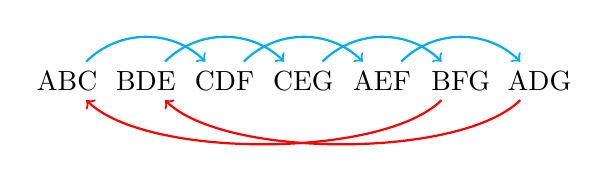
\begin{tikzpicture}
    \node(1) {ABC};
    \node[right of=1] (2) {BDE};
    \node[right of=2] (3) {CDF};
    \node[right of=3] (4) {CEG};
    \node[right of=4] (5) {AEF};
    \node[right of=5] (6) {BFG};
    \node[right of=6] (7) {ADG};
    \draw[->, thick]
    (1) edge[cyan, out=45, in=135, looseness=1,] (3)
    (2) edge[cyan, out=45, in=135, looseness=1,] (4)
    (3) edge[cyan, out=45, in=135, looseness=1,] (5)
    (4) edge[cyan, out=45, in=135, looseness=1,] (6)
    (5) edge[cyan, out=45, in=135, looseness=1,] (7)
    (6) edge[red, out=-135, in=-45, looseness=0.6,] (1)
    (7) edge[red, out=-135, in=-45, looseness=0.6,] (2)
;

\end{tikzpicture}
    \caption{Material transpositions}
    \label{fig:polillas-material-transposition}
\end{figure}

So for a transposition of ABC$\rightarrow$CDF: A maps to C, B maps to D, and C maps to F. In this way, the sequence of events produced by the transposition process is slightly unpredictable as materials do not map directly on to one another. At the beginning of the second sequence, A is mapped to C, but later in that same sequence A maps onto itself.

\begin{table}[H]
    \centering
\resizebox{\columnwidth}{!}{
\begin{tabular}{ c | c c c c c | c c c | c c c c c c | c c c | c c c | c c | c c c }
sections & [01] &  &  &  &  & [02] &  &  & [03] &  & & & & & [04] & & & [05] & & & [06] & & [07] & & \\  
  moments & \textcolor{red}{1}&\textcolor{red}{2} &\textcolor{red}{3} &\textcolor{red}{4} &\textcolor{red}{5} &\textcolor{red}{6} &\textcolor{red}{7} &\textcolor{red}{8} &\textcolor{red}{9} &\textcolor{red}{10} &\textcolor{red}{11} &\textcolor{red}{12} &\textcolor{red}{13} &\textcolor{red}{14} &\textcolor{red}{15} &\textcolor{red}{16} &\textcolor{red}{17} &\textcolor{red}{18} &\textcolor{red}{19} &\textcolor{red}{20} &\textcolor{red}{21}  &\textcolor{red}{22} &\textcolor{red}{23} &\textcolor{red}{24} &\textcolor{red}{25} \\  
  \midrule
  materials & & & & \colorbox{white}{A} & & & & B & & & & & C & E & & \colorbox{white}{A} & & & & & B & A & & &  \\  
 & A & A & B & B & B & D & E & E & C & D & C & C & E & \colorbox{white}{G} & \colorbox{white}{A} & E & E & B & F & F & G & \colorbox{white}{D} & \colorbox{white}{D} & \colorbox{white}{D} & G \\ 
 & & & C & C & & & & & \colorbox{white}{F} & & & & & & F & F & & & & & & G & G & &  \\  
\end{tabular}
}
\caption{Polillas moments part 1}
    \label{fig:p-moments-1}
\end{table}

\begin{table}[H]
    \centering
\resizebox{\columnwidth}{!}{
\begin{tabular}{ c | c c | c c | c c c | c c c | c c c | c c c c | c c | c c | c c c c }
sections & [08] &  & [09] &  & [10] &  &  & [11] &  &  & [12] & & & [13] & & & & [14] & & [15] & & [16] & & & \\  
  moments & \textcolor{red}{26}&\textcolor{red}{27} &\textcolor{red}{28} &\textcolor{red}{29} &\textcolor{red}{30} &\textcolor{red}{31} &\textcolor{red}{32} &\textcolor{red}{33} &\textcolor{red}{34} &\textcolor{red}{35} &\textcolor{red}{36} &\textcolor{red}{37} &\textcolor{red}{38} &\textcolor{red}{39} &\textcolor{red}{40} &\textcolor{red}{41} &\textcolor{red}{42} &\textcolor{red}{43} &\textcolor{red}{44} &\textcolor{red}{45} &\textcolor{red}{46}  &\textcolor{red}{47} &\textcolor{red}{48} &\textcolor{red}{49} &\textcolor{red}{50} \\  
  \midrule
  materials & & & & \colorbox{cyan}{C} & & & & C & & & & & B & F & & \colorbox{yellow}{A} & & & & & A & B & & &  \\  
 & C & C & D & D & C & E & G & G & A & E & B & B & F & \colorbox{yellow}{G} & \colorbox{yellow}{A} & D & D & A & B & B & C & \colorbox{yellow}{D} & \colorbox{yellow}{D} & \colorbox{yellow}{D} & E \\ 
 & & & F & F & & & & & \colorbox{yellow}{F} & & & & & & G & G & & & & & & E & E & &  \\  
\end{tabular}
}
\caption{Polillas moments part 2}
    \label{fig:p-moments-2}
\end{table}

\begin{table}[H]
    \centering
\resizebox{\columnwidth}{!}{
\begin{tabular}{ c | c c c c | c c c c c | c c c | c c c c c | c c c c | c c c c }
sections & [17] &  &  &  & [18] &  &  &  &  & [19] & & & [20] & & & & & [21] & & & & [22] & & & \\  
  moments & \textcolor{red}{51}&\textcolor{red}{52} &\textcolor{red}{53} &\textcolor{red}{54} &\textcolor{red}{55} &\textcolor{red}{56} &\textcolor{red}{57} &\textcolor{red}{58} &\textcolor{red}{59} &\textcolor{red}{60} &\textcolor{red}{61} &\textcolor{red}{62} &\textcolor{red}{63} &\textcolor{red}{64} &\textcolor{red}{65} &\textcolor{red}{66} &\textcolor{red}{67} &\textcolor{red}{68} &\textcolor{red}{69} &\textcolor{red}{70} &\textcolor{red}{71}  &\textcolor{red}{72} &\textcolor{red}{73} &\textcolor{red}{74} &\textcolor{red}{75} \\  
  \midrule
  materials & & & & \colorbox{pink}{A} & & & & \colorbox{pink}{B} & & & & & A & B & & B & & & & & \colorbox{cyan}{C} & C & & &  \\  
 & \colorbox{pink}{A} & \colorbox{pink}{A} & E & E & \colorbox{pink}{B} & F & \colorbox{yellow}{G} & \colorbox{yellow}{G} & \colorbox{yellow}{A} & \colorbox{pink}{D} & A & A & \colorbox{cyan}{B} & C & B & \colorbox{yellow}{D} & \colorbox{yellow}{D} & C & D & D & F & \colorbox{cyan}{E} & \colorbox{cyan}{E} & E & \colorbox{pink}{G} \\ 
 & & & \colorbox{yellow}{F} & \colorbox{yellow}{F} & & & & & G & & & & & & E & \colorbox{orange}{E} & & & & & & \colorbox{pink}{G} & \colorbox{pink}{G} & &  \\  
\end{tabular}
}
\caption{Polillas moments part 3}
    \label{fig:p-moments-3}
\end{table}

In the figures above, yellow highlights refer to materials in the same position as the preceding transposition. Blue highlights refer to materials in the same point in time but not the same vertical position as the preceding transposition. Pink highlights refer to materials in the same position as the original transposition. Red highlights refer to materials in the same point in time but not the same vertical position as the original transposition.

\subsection{Material A}

Material \boxed{\text{A}} consists primarily of gestured derived from glissando motions. I sketched seven available manifestations of the material, not all of which occur in the final work. The narrative arc of this material was meant to be the gradual revelation of higher partials of the fundamental provided by open strings across the ensemble. The open strings were chosen so that no instrument would have octavations of the same harmonic series. I also wanted to avoid a common trope which occurs when many natural harmonics are used in a work. It can be difficult to avoid the impression of the stack of perfect fifths representing the tuning of the strings of each instrument. By retuning the cello's \textit{IV} string from C\mynatural \hspace{0.12cm}to a lower B\myflat, I was able to create a whole-tone chord voiced entirely with open strings. Several other materials feature a significant manifestation where the glissando motion has infected the pre-established nature of the material. This is never the product of a \textit{ligature} material juxtaposition, as if material \boxed{\text{A}} and another material were listed as being performed simultaneously in the form diagram, rather the glissandi represent a doppelgänger effect of convergent evolution.

\begin{enumerate}
\item damped glissando
\item damped trills with shallow gliss
\item natural harmonic gliss (B\myflat1 C\mynatural3 D\mynatural4 E\mynatural5)
\item sustain + unidirectional gliss (intentionally rhythmic) slow$\rightarrow$fast, norm$\rightarrow$circular bow, 
\item \textcolor{red}{x} bow contact points + gliss: same bowing + different rhythm OR same rhythm + different bowing
\item glissando tremolo — shallow gliss: change string contact point, change tremolo speed, talea with intermittent short durations to anchor tremolo
\item flautando full bows
\end{enumerate}

\subsection{Material B}

Material \boxed{\text{B}} develops in two different directions. One aspect of \boxed{\text{B}} is the harmonic language and the other is the bowing technique used at the opening of the work. One developmental trajectory is the gradual slowing of individual spazzolato articulations, developing from swipes of barely audible pitch to perforated sounds of crunching bow hair. The other is the gradual crystallization of rigorous harmonic manipulations, almost always formalized as ratios above a fundamental even when notated as quarter tones. These trajectories result in two culminations from measures 188-210 and 258-273 respectively.

\begin{enumerate}
\item talea — repeat pitches by group
\item sputtering — potamia
\item grand interpolation (scratch$\rightarrow$normale$\rightarrow$slow bow$\rightarrow$\ac{XSB}) — voice-led from previous
\item chorale — Just Intonation Tonnetz voice-led by hand
\end{enumerate}

\subsection{Material C}\label{material-C-summary}

\boxed{\text{C}} is a mostly static material. The pitch process in these materials is usually static with occasional voice-leading. The rhythmic language is polyrhythmic. Each voice is given a different prolation value and talea of a long value followed by a short value. The short value is used to accent the polyrhythm as an anchor point for an articulation such as an accent, tremolo, or circular bowing.

\begin{enumerate}
\item sustain with intermittent accent, tremolo, gliss
\item tremolo$\rightarrow$circular bowing$\rightarrow$normale
\item tremolo with \lilyTimeSignature{1}{6} metric interruption circular bowings
\item \textcolor{red}{x} cascading spatial notation
\end{enumerate}

\subsection{Material D}

Material \boxed{\text{D}} is represented by various trills. The trills are mostly used as a method whereby the duration of each measure is clearly heard. The trill gestures are almost always proportionally related directly to the measure duration. The pitch material is derived from traditional serial pitch manipulation but eventually develops as a sliding glissando figure in contrary motion.

\begin{enumerate}
\item unision attacks
\item cascades
\item duets
\item \textcolor{red}{x} grace-note anticipations
\end{enumerate}

\subsection{Material E}

\boxed{\text{E}} is similar to \textit{Akasha}'s microtonal polyphony material. The main identifying feature of \boxed{\text{E}} is the use of explicitly notated bow speeds in the form of bow contact point fractions. This produces incredibly unique and unevenly distributed bowing colors of varying degrees of scratch and flautando. The harmony features stepwise motion in quarter-tonal pitch space. Occasionally these stepwise quarter tones are derived from voicings of the harmonic spectrum. Local dynamic trajectories are also a key element.

\begin{enumerate}
\item frozen + grand interpolation / suddenly removed: accumulate divisions $\frac{7}{8}, \frac{1}{8}, \frac{9}{8}, \frac{2}{8}$ talea
\item growth or ``manifest'': gradually accelerate
\item revisit stage 1 with explicit bow contact points: \ac{XSB}$\rightarrow$slow bow$\rightarrow$ordinario$\rightarrow$flautando
\item reverse stage 2
\end{enumerate}

\subsection{Material F}

\boxed{\text{F}} is characterized as the staccato material. Sometimes taking the form of gettati and sometimes taking the form of tight, violent attacks, the general harmonic trajectory is infinite ascension of the same repeating motif. Variation is produced by the rhythmic material and type of attack used to produce each sound. 

\begin{enumerate}
\item clock ticks
\item hocketted, voice-led, stepwise melody
\item gettato that sometimes goes behind the bridge
\item grand interpolation, ascending like \textit{Akasha}, dense$\rightarrow$sparse
\item gettati$\rightarrow$multi-staccati
\item feather-beam gettato repeat x6
\end{enumerate}

\subsection{Material G}

Finally material \boxed{\text{G}} is mostly performed by bowing directly on the wood of the bridge. Occasionally, the bow drifts away from the wood in either direction, once leading to bowing behind the bridge, and ending the piece bright, shimmering overtones. The rhythmic material is usually a very simple, repeating talea, but occasionally is produced by an accumulation of attack density with an even-division rhythm maker.

\begin{enumerate}
\item shrieks, bowed on wrapping, sparse$\rightarrow$dense
\item white noise, \lilyDynamics{ppp}, occasional tremolo
\item revisit stage 2 + \ac{CLT}
\item revisit stage 2 + occasional gettato
\item revisit stage 1 + dense$\rightarrow$sparse
\item bow on the body of the instrument
\end{enumerate}

\begin{figure}[p]
    \centering
    \rotatebox{90}{
    \resizebox{!}{\textwidth}{
\begin{tikzpicture}[
node distance = 25mm and 15mm,
every edge quotes/.style = {font=\footnotesize, rectangle, draw, fill=white}
                    ]
    \node(1) {$40$};
    \node[right of=1] (2) {$60$};
    \node[right of=2] (3) {$66 \frac{2}{3}$};
    \node[right of=3] (4) {{72}};
    \node[right of=4] (5) {{90}};
    \node[right of=5] (6) {{120}};
    \node[right of=6] (7) {{130}};
    \draw[->, thick]
    (1) edge[red, out=45, in=135, looseness=2, "4:13"] (7)
    
    (1) edge[red, out=45, in=135, looseness=2, "1:3"] (6)
    (2) edge[red, out=45, in=135, looseness=2, "6:13"] (7)

    (1) edge[red, out=45, in=135, looseness=2, "4:9"] (5)
    (2) edge[red, out=45, in=135, looseness=2, "1:2"] (6)
    (3) edge[red, out=45, in=135, looseness=2, "20:39"] (7)

    (1) edge[red, out=45, in=135, looseness=2, "5:9"] (4)
    (2) edge[red, out=45, in=135, looseness=2, "2:3"] (5)
    (3) edge[red, out=45, in=135, looseness=2, "5:9"] (6)
    (4) edge[red, out=45, in=135, looseness=2, "36:65"] (7)

    (1) edge[red, out=45, in=135, looseness=2, "3:5"] (3)
    (2) edge[red, out=45, in=135, looseness=2, "5:6"] (4)
    (3) edge[red, out=45, in=135, looseness=2, "20:27"] (5)
    (4) edge[red, out=45, in=135, looseness=2, "3:5"] (6)
    (5) edge[red, out=45, in=135, looseness=2, "9:13"] (7)

    (1) edge[red, out=45, in=135, looseness=2, "2:3"] (2)
    (2) edge[red, out=45, in=135, looseness=2, "9:10"] (3)
    (3) edge[red, out=45, in=135, looseness=2, "25:27"] (4)
    (4) edge[red, out=45, in=135, looseness=2, "4:5"] (5)
    (5) edge[red, out=45, in=135, looseness=2, "3:4"] (6)
    (6) edge[red, out=45, in=135, looseness=2, "12:13"] (7);

    \draw[<-, thick]
    (1) edge[cyan, out=-45, in=-135, looseness=2, "13:4"] (7)
    
    (1) edge[cyan, out=-45, in=-135, looseness=2, "3:1"] (6)
    (2) edge[cyan, out=-45, in=-135, looseness=2, "13:6"] (7)

    (1) edge[cyan, out=-45, in=-135, looseness=2, "9:4"] (5)
    (2) edge[cyan, out=-45, in=-135, looseness=2, "2:1"] (6)
    (3) edge[cyan, out=-45, in=-135, looseness=2, "39:20"] (7)

    (1) edge[cyan, out=-45, in=-135, looseness=2, "9:5"] (4)
    (2) edge[cyan, out=-45, in=-135, looseness=2, "3:2"] (5)
    (3) edge[cyan, out=-45, in=-135, looseness=2, "9:5"] (6)
    (4) edge[cyan, out=-45, in=-135, looseness=2, "65:36"] (7)

    (1) edge[cyan, out=-45, in=-135, looseness=2, "5:3"] (3)
    (2) edge[cyan, out=-45, in=-135, looseness=2, "6:5"] (4)
    (3) edge[cyan, out=-45, in=-135, looseness=2, "27:20"] (5)
    (4) edge[cyan, out=-45, in=-135, looseness=2, "5:3"] (6)
    (5) edge[cyan, out=-45, in=-135, looseness=2, "13:9"] (7)

    (1) edge[cyan, out=-45, in=-135, looseness=2, "3:2"] (2)
    (2) edge[cyan, out=-45, in=-135, looseness=2, "10:9"] (3)
    (3) edge[cyan, out=-45, in=-135, looseness=2, "27:25"] (4)
    (4) edge[cyan, out=-45, in=-135, looseness=2, "5:4"] (5)
    (5) edge[cyan, out=-45, in=-135, looseness=2, "4:3"] (6)
    (6) edge[cyan, out=-45, in=-135, looseness=2, "13:12"] (7)
    ;

\end{tikzpicture}
}
}
    \caption{Tempo Map}
    \label{fig:apolillas-tempo}
\end{figure}

\begin{figure}[p]
\centering
    \rotatebox{90}{
    \resizebox{!}{0.9\textwidth}{
    \includegraphics[width=6in,page=1]{lilypond/polillas_graph.pdf}
}
}
    \caption{Page 1 of the color-coded graph of the large-scale form of Polillas}
    \label{fig:Polillas-graph-1}
\end{figure}

\begin{figure}[p]
\centering
    \rotatebox{90}{
    \resizebox{!}{0.9\textwidth}{
    \includegraphics[width=6in,page=2]{lilypond/polillas_graph.pdf}
    }
    }
    \caption{Page 2 of the color-coded graph of the large-scale form of Polillas}
    \label{fig:Polillas-graph-2}
\end{figure}

\subsection{Tempo}

A technique I derived from Bača's composition \textit{(HARMONY)}, for narrator and nine players, was the formulation of a reservoir of tempi. These tempi originated from a specific sequence of metric modulations. I produced a graph of all of the ratio relationships between each tempo in order to be able to modulate from one speed to any other in the reservoir. In actual practice, these modulations are not foreshadowed by an anchoring rhythm which crosses the boundary of the modulation, rather they are abrupt changes of speed. See figure \ref{fig:apolillas-tempo}.

Another possible embedding of this map is as a complete graph as seen in figure \ref{fig:polillas-tempo-2}. The only tempo which exists outside of the standard modulatory system is 108. I decided that this tempo was to be considered a ``dead end.'' The only way to modulate to or from 108 is through 90.

\begin{figure}
    \centering
\begin{tikzpicture}
  \graph[clique, n=7, clockwise, radius=2cm]
  {
    1/"$40$", 2/"$60$", 3/"$66\frac{2}{3}$", 4/"$72$", 5/"$90$", 6/"$120$", 7/"$130$"
  };
  \node[left of=5] (8) {$108$};
  \draw[<->]
  (5) edge[red, out=180, in=0, looseness=2, "$6:5$"] (8);
\end{tikzpicture}
    \caption{Alternate embedding of Tempo relationships as a complete graph}
    \label{fig:polillas-tempo-2}
\end{figure}

\section{Interpretation of Outline}

The interpretation of the three-layered outline was totally free. Generally the central line was to be considered as the foreground and the upper and lower lines were to be considered background counterpoint. At each moment, I decided what type of relationship concurrent materials should share.

While it is unlikely that the piece can be audibly interpreted as a binary, the second page of the color-coded graph reveals more oppositional relationships. I wanted the music after the large chorale section to somehow disintegrate due to its own futility. Materials are always interrupted and don't see culmination until the emergence of traditional beauty at the end of the work, drawn out of the originally toneless bridge material, only to be pull away: denying resolution in the final breath of the piece. By defining the materials and their developmental trajectories in the abstract, I was able to specify and implement various developments and transitions and to structurally distribute them where I believed they would be most effective.

\section{Conclusion}

In Polillas, I developed my own version of a combination of processes developed by Francisco Guerrero and Trevor Bača. As a user of the Abjad \ac{API} for \ac{FSC}, I inherit more explicitly from works like \textit{Akasha}. However, much of the same types of formalizations and combinatorial practices exist within my compositions as well. These techniques were further developed in my sinfonietta \textit{Alu} by way of the expanded capabilities for counterpoint in the large, diverse ensemble setting.\footnote{The complete source code for \textit{Polillas} can be found at \url{https://github.com/GregoryREvans/polillas}} 